%%%%%%%%%%%%%%%%%%%%%%%%%%%%%%%%%%%%%%%%%%%%%%%%%%%%%%%%%%%%%%%%%%%%%%%%%%%%%%%%%%%%%%%%µ%%%%%%%%%%%
%%%  Improving Schema Matching with Linked Data %%%%
%%%%%%%%%%%%%%%%%%%%%%%%%%%%%%%%%%%%%%%%%%%%%%%%%%%%%%%%%%%%%%%%%%%%%%%%%%%%%%%%%%%%%%%%%%%%%%%%%%%%

\documentclass{sig-alternate}

\usepackage{amssymb}
\usepackage{amsmath}
\usepackage{graphicx}
\usepackage{tabularx}
\graphicspath{ {Figures/} }


\begin{document}

\title{Improving Schema Matching with Linked Data}

\author{
\alignauthor
Ahmad Assaf, Eldad Louw, Aline Senart, Corentin Follenfat and David Trastour\\
       \affaddr{SAP Research, SAP Labs France SAS}\\
       \affaddr{805 avenue du Dr. Maurice Donat, BP 1216}\\
       \affaddr{06254 Mougins Cedex, France}\\
       \email{firstname.lastname@sap.com}
\and
\alignauthor
Rapha\"el Troncy \\
       \affaddr{EURECOM}\\
       \affaddr{06904 Sophia Antipolis Cedex, France}\\
       \email{raphael.troncy@eurecom.fr}
}
\maketitle

%%%%%%%%%%%%%%%%%%%%%%%%%%%%%%%
%%%  Beginning of document  %%%
%%%%%%%%%%%%%%%%%%%%%%%%%%%%%%%

\begin{abstract}
With today's public data sets containing billions of data items, more and more companies are looking to integrate external data with their traditional enterprise data to improve business intelligence analysis. These distributed data sources however exhibit heterogeneous data formats and terminologies and may contain noisy data. In this paper, we present a novel framework that enables business users to semi-automatically perform data integration on potentially noisy tabular data. This framework offers an extension to Google Refine with novel schema matching algorithms leveraging Freebase rich types. First experiments show that using Linked Data to map cell values with instances and column headers with types improves significantly the quality of the matching results and therefore should lead to more informed decisions.
\end{abstract}

%%%%%%%%%%%%%%%%%%%%%%%%%%%%%%%
%%%  Introduction  %%%
%%%%%%%%%%%%%%%%%%%%%%%%%%%%%%%

\section{Introduction}

Companies have traditionally performed business analysis based on transactional data stored in legacy relational databases. The enterprise data available for decision makers was typically relationship management or enterprise resource planning data~\cite{Hernandez:2013:DDM:2462633}. However social media feeds, weblogs, sensor data, or data published by governments or international organizations are nowadays becoming increasingly available~\cite{citeulike:9784019}.

The quality and amount of structured knowledge available make it now feasible for companies to mine this huge amount of public data and integrate it in their next-generation enterprise information management systems. Analyzing this new type of data within the context of existing enterprise data should bring them new or more accurate business insights and allow better recognition of sales and market opportunities~\cite{bigData}.

These new distributed sources, however, raise tremendous challenges. They have inherently different file formats, access protocols or query languages. They possess their own data model with different ways of representing and storing the data. Data across these sources may be noisy (e.g. duplicate or inconsistent), uncertain or be semantically similar yet different~\cite{kavitha}. Integration and provision of a unified view for these heterogeneous and complex data structures therefore require powerful tools to map and organize the data.

In this paper, we present a framework that enables business users to semi-automatically combine potentially noisy data residing in heterogeneous silos. Semantically related data is identified and appropriate mappings are suggested to users. On user acceptance, data is aggregated and can be visualized directly or exported to Business Intelligence reporting tools. The framework is composed of a set of extensions to Google Refine server and a plug-in to its user interface\footnote{http://code.google.com/p/google-refine/}. Google Refine was selected for its extensibility as well as good cleansing and transformation capabilities~\cite{bizer_linked_2009}.

We first map cell values with instances and column headers with types from popular data sets from the Linked Open Data Cloud. To perform the matching, we use the Auto Mapping Core (also called AMC~\cite{conf/icde/PeukertER12}) that combines the results of various similarity algorithms. The novelty of our approach resides in our exploitation of Linked Data to improve the schema matching process. We developed specific algorithms on rich types from vector algebra and statistics. The AMC generates a list of high-quality mappings from these algorithms allowing better data integration.

First experiments show that Linked Data increases significantly the number of mappings suggested to the user. Schemas can also be discovered if column headers are not defined and can be improved when they are not named or typed correctly. Finally, data reconciliation can be performed regardless of data source languages or ambiguity. All these enhancements allow business users to get more valuable and higher-quality data and consequently to take more informed decisions.

The rest of the paper is organized as follows. Section 2 presents some related work. Section 3 describes the framework that we have designed for business users to combine data from heterogeneous sources. Section 4 validates our approach and shows the value of the framework through experiments. Finally, Section 5 concludes the paper and discusses future work.

%%%%%%%%%%%%%%%%%%%%%%%%%%%%%%%
%%%  Related Work  %%%
%%%%%%%%%%%%%%%%%%%%%%%%%%%%%%%

\section{Related Work}

While schema matching has always been an active research area in data integration, new challenges are faced today by the increasing size, number and complexity of data sources and their distribution over the network. Data sets are not always correctly typed or labeled and that hinders the matching process.

In the past, some work has tried to improve existing data schemas~\cite{ DBLP:journals/debu/MillerA03} but literature mainly covers automatic or semi-automatic labeling of anonymous data sets through Web extraction. Examples include~\cite{cas04} that automatically labels news articles with a tree structure analysis or~\cite{wang2003extraction} that defines heuristics based on distance and alignment of a data value and its label. These approaches are however restricting label candidates to Web content from which the data was extracted.~\cite{DBLP:conf/otm/SilvaBCS07} goes a step further by launching speculative queries to standard Web search engines to enlarge the set of potential candidate labels. More recently,~\cite{Limaye:2010:ASW:1920841.1921005} applies machine learning techniques to respectively annotate table rows as entities, columns as their types and pairs of columns as relationships, referring to the YAGO ontology. The work presented aims however at leveraging such annotations to assist semantic search queries construction and not at improving schema matching.

With the emergence of the Semantic Web, new work in the area has tried to exploit Linked Data repositories. The authors of~\cite{Syed2010Tables} present techniques to automatically infer a semantic model on tabular data by getting top candidates from Wikitology~\cite{conf/aaaiss/FininSMMP09} and classifying them with the Google page ranking algorithm. Since the authors' goal is to export the resulting table data as Linked Data and not to improve schema matching, some columns can be labeled incorrectly, and acronyms and languages are not well handled~\cite{Syed2010Tables}. In the Helix project~\cite{conf/www/HassanzadehDFKSW11}, a tagging mechanism is used to add semantic information on tabular data. A sample of instances values for each column is taken and a set of tags with scores are gathered from online sources such as Freebase\footnote{http://www.freebase.com/}. Tags are then correlated to infer annotations for the column. The mechanism is quite similar to ours but the resulting tags for the column are independent of the existing column name and sampling might not always provide a representative population of the instance values.

%%%%%%%%%%%%%%%%%%%%%%%%%%%%%%%
%%%  Proposition  %%%
%%%%%%%%%%%%%%%%%%%%%%%%%%%%%%%

\section{Proposition}

Google Refine (formerly Freebase Gridworks) is a tool designed to quickly and efficiently process, clean and eventually enrich large amounts of data with existing knowledge bases such as Freebase. The tool has however some limitations: it was initially designed for data cleansing on only one data set at a time, with no possibility to compose columns from different data sets. Moreover, Google Refine has some strict assumptions over the input of spreadsheets which makes it difficult to identify primitive and complex data types.
The AMC is a novel framework that supports the construction and execution of new matching components or algorithms. AMC contains several matching components that can be plugged and used, like string matchers (Levenshtein, JaroWinkler\dots  etc.), data types matchers and path matchers. It also provides a set of combination and selection algorithms to produce optimized results (weighted average, average, sigmoid\dots  etc.).
In this section, we describe in detail our framework allowing data mashup from several sources. We first present our framework architecture, then the activity flow and finally our approach to schema matching.

%%%%%%%%%%%%%%%%%%%%%%%%%%%%%%%
%%%  Framework Architecture  %%%
%%%%%%%%%%%%%%%%%%%%%%%%%%%%%%%

\subsection{Framework Architecture}
Google Refine makes use of a modular web application framework similar to OSGi called Butterfly\footnote{http://code.google.com/p/simile-butterfly/}. The server-side written in Java maintains states of the data (undo/redo history, long-running processes, etc.) while the client-side implemented in Javascript maintains states of the user interface (facets and their selections, view pagination, etc.). Communication between the client and server is done through REST web services.

\begin{figure}[ht!]
  \centering
    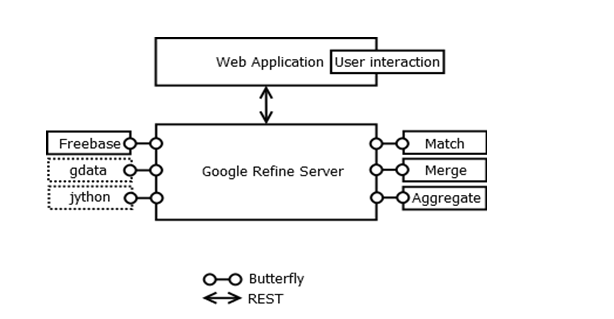
\includegraphics[scale=0.6]{architecture-1.png}
  \caption{Framework Architecture}
  \label{fig:framework_architecture}
\end{figure}

As depicted in \ref{fig:framework_architecture}, our framework leverages Google Refine and defines three new Butterfly modules to extend the server's functionality (namely Match, Merge and Aggregate modules) and one JavaScript extension to capture user interaction with these new data matching capabilities.

\subsection{Activity Flow}
This section presents the sequence of activities and interdependencies between these activities when using our framework. \ref{fig:Activity_workflow} gives an outline of these activities.

\begin{figure}[ht!]
  \centering
    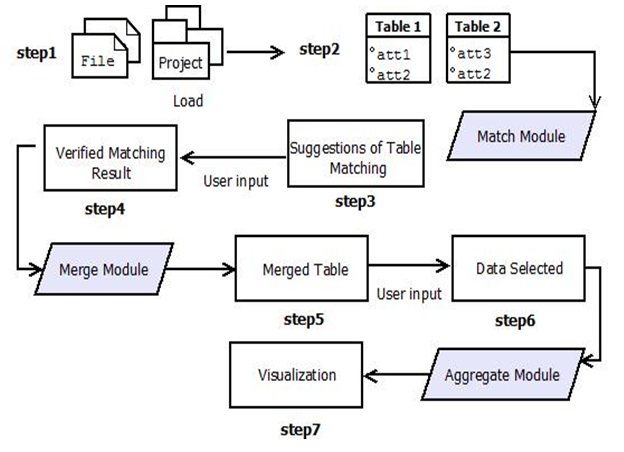
\includegraphics[scale=0.4]{architecture-2.png}
  \caption{Activity Workflow}
  \label{fig:Activity_workflow}
\end{figure}

The data sets to match can be contained in files (e.g. csv, Excel spreadsheets, etc.) or defined in Google Refine projects (step 1). The inputs for the match module are the source and target files and/or projects that contain the data sets. These projects are imported into the internal data structure (called schema) of the AMC~\cite{5767940} (step 2). The AMC then uses a set of built-in algorithms to calculate similarities between the source and target schemas on an element basis, i.e. column names in the case of spreadsheets or relational databases. The output is a set of similarities, each containing a triple consisting of source schema element, target element, and similarity between the two.

These results are presented to the user in tabular form (step 3) such that s/he can check, correct, and potentially complete the mappings (step 4).

Once the user has completed the matching of columns, the merge information is sent back to Google Refine, which calls the merge module. This module creates a new project, which contains a union of the two projects where the matched columns of the target project are appended to the corresponding source columns (step 5). The user can then select the columns that s/he wants to merge and visualize by dragging and dropping the required columns onto the fields that represent the x and y axes (step 6).

Once the selection has been performed, the aggregation module merges the filtered columns and the result can then be visualized (step 7). As aggregation operations can quickly become complex, our default aggregation module can be replaced by more advanced analytics on tabular data. The integration of such a tool is part of future work.

\subsection{Schema Matching }
Schema matching is typically used in business to business integration, metamodel matching, as well as Extract, Transform, Load (ETL) processes. For non-IT specialists the typical way of comparing financial data from two different years or quarters, for example, would be to copy and paste the data from one Excel spreadsheet into another one, thus creating reduncancies and potentially introducing copy-and-paste errors. By using schema matching techniques it is possible to support this process semi-automatically, i.e. to determine which columns are similar and propose them to the user for integration. This integration can then be done with appropriate business intelligence tools to provide visualisations.

One of the problems in performing the integration is the quality of data. The columns may contain data that is noisy or incorrect. There may also be no column headers to provide suitable information for matching. A number of approaches exploit the similarities of headers or similarities of types of column data. We propose a new approach that exploits semantic rich typing provided by popular datasets from the Linked Data cloud.


\subsection{Data Reconciliation}
Reconciliation enables entity resolution, i.e. matching cells with corresponding typed entities in case of tabular data. Google Refine already supports reconciliation with Freebase but requires confirmation from the user. For medium to large data sets, this can be very time-consuming. To reconcile data, we therefore first identify the columns that are candidates for reconciliation by skipping the columns containing numerical values or dates. We then use the Freebase search API to query for each cell of the source and target columns the list of typed entities candidates. Results are cached in order to be retrieved by our similarity algorithms.


\subsection{Matching Unnamed and Untyped Columns}
The AMC has the ability to combine the results of different matching algorithms. Its default built-in matching algorithms work on column headers and produce an overall similarity score between the compared schema elements. It has been proven that combining different algorithms greatly increases the quality of matching results~\cite{conf/icde/PeukertER12}\cite{conf/wise/StracciaT05}. However, when headers are missing or ambiguous, the AMC can only exploit domain intersection and inclusion algorithms based on column data. We have therefore implemented three new similarity algorithms that leverage the rich types retrieved from Linked Data in order to enhance the matching results of unnamed or untyped columns. They are presented below.


\subsubsection{Cosine Similarity}
The first algorithm that we implemented is based on vector algebra. Let $v$ be the vector of ranked candidate types returned by Freebase for each cell value of a column. Then:
\[v:=\sum^K_{i=1}{a_i}*\overrightarrow{t_i}\]
where $a_i$ is the score of the entry and $\overrightarrow{t_i}$ is the type returned by Freebase. The vector notation is chosen to indicate that each distinct answer determines one dimension in the space of results.

Each cell value has now a weighted result set that can be used for aggregation to produce a result vector for the whole column. The column result $V$ is then given by:
\[V?\sum^n_{i=1}{v_i}\]
We compare the result vector of candidate types from the source column with the result vector of candidate types from the target column. Let $W$ be the result vector for the target column, then the similarity $s$ between the columns pair can be calculated using the absolute value of the cosine similarity function:
\[s?\frac{\left|(V*W)\right|}{\left\|V\right\|*\left\|W\right\|}\]


\subsubsection{Pearson Product-Moment Correlation Coefficient (PPMCC)}

The second algorithm that we implemented is PPMCC, a statistical measure of the linear independence between two variables $\left(x,y\right)$~\cite{citeulike:8051946}. In our method, x is an array that represents the total scores for the source column rich types, y is an array that represents the mapped values between the source and the target columns. The values present in x but not in y are represented by zeros. We have:
\[SourceColumn\ \left[\left\{R_1,C_{sr1}\right\},\left\{R_2,C_{sr2}\right\},\left\{R_3,C_{sr3}\right\}\dots \ \left\{R_n,C_{srn}\right\}\right]\]
\[TargetColumn\ \left[\left\{R_1,C_{tr1}\right\},\left\{R_2,C_{tr2}\right\},\left\{R_3,C_{tr3}\right\}\dots \ \left\{R_n,C_{trn}\right\}\right]\]
Where $R_1,\ R_{2,}{\dots ,R}_n$ are different rich type values retrieved from Freebase, $C_{sr1},\ C_{sr2},\dots ,\ C_{srn}$ are the sum of scores for each corresponding r occurrence in the source column, and $C_{tr1},\ C_{tr2},\ \dots ,\ C_{trn}$ are the sum of scores for each corresponding r occurrence in the target column.

The input for PPMC consists of two arrays that represent the values from the source and target columns, where the source column is the column with the largest set of rich types found. For example:
\[X=\ \left[C_{sr1},C_{sr2},C_{sr4},\ \dots ,\ C_{srn}\right]\]
\[Y=\ \left[0,C_{tr2},C_{tr4},\ \dots ,\ C_{trn}\right]\]
Then the sample correlation coefficient (r) is calculated using:
\[r=\ \frac{\sum^n_{i=1}{\left(x_i-\ \overline{x}\right)\left(y_{i\ }-\ \overline{y}\right)}}{\sqrt{\sum^n_{i=1}{{\left(x_i-\ \overline{x}\right)}^{2\ }}}\sqrt{\sum^n_{i=1}{{\left(y_i-\ \overline{y}\right)}^2}}}\ \]
Based on a sample paired data$\left(x_i,y_i\right)$, the sample PPMCC is:
\[r=\ \frac{1}{n-1}\sum^n_{i=1}{\left(\frac{x_i-\ \overline{x}}{s_x}\right)}\left(\frac{y_i-\ \overline{y}}{s_y}\right)\]
Where $\left(\frac{x_i-\ \overline{x}}{s_x}\right),\ \overline{x\ }$and $s_x$ are the standard score, sample mean and sample standard deviation, respectively.


\subsubsection{Spearman's Rank Correlation Coefficient}
The last algorithm that we implemented to match unnamed and untyped columns is Spearman's rank correlation coefficient~\cite{books/daglib/0020904}. It applies a rank transformation on the input data and computes PPMCC afterwards on the ranked data. In our experiments we used Natural Ranking with default strategies for handling ties and NaN values. The ranking algorithm is however configurable and can be enhanced by using more sophisticated measures.


\subsection{Column Labeling}
We showed in the previous section how to match unnamed and untyped columns. Column labeling is however beneficial as the results of our previous algorithms can be combined with traditional header matching techniques to improve the quality of matching.

Rich types retrieved from Freebase are independent from each other. We need to find a method that will determine normalized score for each type in the set by balancing the proportion of high scores with the lower ones. We used Wilson score interval for a Bernoulli parameter that is presented in the following equation:
\[w={\left(\widehat{p\ }+\ \frac{z^2_{{\alpha }/{2}}}{2n}\  \begin{array}{c}
+ \\
- \end{array}
z_{{\alpha }/{2}}\sqrt{{\left[\hat{p}\left(1-\ \hat{p}\right)+\ {z^2_{{\alpha }/{2}}}/{4n}\right]}/{n}}\ \ \ \right)}/{\left(1+{z^2_{{\alpha }/{2}}}/{n}\right)}\]
Here $\hat{p}$ is the average score for each rich type, n is the total number of scores and $z_{{\alpha }/{2}}$ is the score level; in our case it is 1.96 to reflect a score level of 0.95.

\subsection{Handling Non-String Values}
So far, we have covered several methods to identify the similarity between ``String'' values, but how about other numeral values such as dates, money, distance,etc.? For this purpose, we have implemented some basic type identifier that can recognize dates, money, numerical values, numerals used as identifiers. This will help us in better match corresponding entries. Adjusting AMC's combination algorithms can be of great importance at this stage. For example, assigning weights to different matchers and tweaking the configuration can yield more accurate results.


%%%%%%%%%%%%%%%%%%%%%%%%%%%%%%%
%%%  Experiments  %%%
%%%%%%%%%%%%%%%%%%%%%%%%%%%%%%%

\section{Experiments}
We present in this section results from experiments we conducted using the different methods described above. To appreciate the value of our approach, we have used a real life scenario that exposes common problems faced by the management in SAP. The data we have used come from two different SAP systems: the Event tracker and the Travel Expense Manager.

The Event Tracker provides an overview of events (Conferences, Internal events, etc.) that SAP Research employees contribute to or host. The entries in this system contain as much information as necessary to give an overview of the activity like the activity type and title, travel destination, travel costs divided into several sub categories (conference fees, accommodation, transportation and others), and duration related information (departure, return dates). Entries in the Event Tracker are generally entered in batches as employees fill in their planned events that they wish to attend or contribute to at the beginning of each year. Afterwards, managers can either accept or reject these planned events according to their allocated budget.

On the other hand, the Travel Expense Manager contains the actual expenses data for the successfully accepted events. This system is used by employees to enter their actual trip details in order to claim their expenses. It contains more detailed information and aggregated views of the events, such as the total cost, duration calculated in days, currency exchange rates and lots of internal system tags and identifiers.

Matching reports from these two systems is of great benefit to managers to organize and monitor their allocated budget. They mainly want to:

\begin{enumerate}
\item  Find the number of the actual (accepted) travels compared with the total number of entered events.

\item  Calculate the deviation between the estimated and actual cost of each event.
\end{enumerate}

However, matching from these two sources can face several difficulties that can be classified in two categories: column headers and cells. Global labels (or column headers as we are dealing with spreadsheet files) can have the following problems:

\begin{enumerate}
\item  Missing labels: importing files into Google Refine with empty headers will result in assigning that column a dummy name by concatenating the word ``column'' with a number starting from 0.

\item  Dummy labels or semantically unrelated names: this is a common problem especially from the data coming from the Travel Expense Manager. This can be applied to columns that are labeled according to the corresponding database table (i.e. lbl\_dst to denote destination label). Moreover, column labels do not often convey the semantic type of the underlying data.
\end{enumerate}

The second category of difficulties is at cell (single entry) level:

\begin{enumerate}
\item  Detecting different date formats: we have found out that dates field coming from the two systems have different formats. Moreover, the built-in type detection in Google Refine converts detected date into another third format.

\item  Entries from different people can be made in different languages.

\item  Entries in the two systems can be incomplete, an entry can be shortened automatically by the system. For example, selecting a country in the Travel Expense Manager will result in filling out that country code in the exported report (i.e. France = FR).

\item  Inaccurate entries: this is one of the most common problems. Users enter sometimes several values in some fields that correspond to the same entity. For example, in the destination column, users can enter the country, the airport at the destination, the city or even the exact location of the event (i.e. office location).
\end{enumerate}

The data used in our evaluation consists of around 60 columns and more than 1000 rows. Our source data set will be the data coming from Event Tracker, and our target data set will be the data from the Travel Expense Manager.

By manually examining the two data sets, we have found out that most of the column headers in the source table exist and adequately present the data. However, we have noticed few missing labels in the target table and few ambiguous column headers. We have detected several entries in several languages: the main language is English but we have also identified French, German. Destination field had entries in several formats: we have noticed airport names, airports by their IATA code, country codes, and cities.

Running AMC with its default matchers returns the matching results shown in Table \ref{tab:Similarity_Scores_Using_the_AMC_Default_Matching_Algorithms}.

\begin{table}[ht]
\centering
\begin{tabular}{|c|c|c|} \hline
\textbf{Source Column} & \textbf{Target Column} & \textbf{Similarity Score} \\ \hline
Reason for Trip & Reason for Trip & 1 \\ \hline
Begins On & Trip Begins On & 0.8333334 \\ \hline
Ends On & Trip Ends On & 0.8 \\ \hline
Total & Total Cost & 0.7333335 \\ \hline
Trip & Trip Destination & 0.72727275 \\ \hline
Amount & Receipt Amount & 0.7142875 \\ \hline
Pd by Comp & Paid by Company & 0.6904762 \\ \hline
Period & Period Number & 0.6666667 \\ \hline
Pers.No. & Sequential no. & 0.5555556 \\ \hline
M/Km & Total Miles/Km & 0.55 \\ \hline
Curr. & Currency & 0.5 \\ \hline
Crcy & Currency & 0.5 \\ \hline
\end{tabular}
\caption{Similarity Scores Using the AMC Default Matching Algorithms}
\label{tab:Similarity_Scores_Using_the_AMC_Default_Matching_Algorithms}
\end{table}

The AMC has perfectly matched the two columns labeled ``Reason for Trip'' using name and data type similarity calculations (the type here was identified as a String). Moreover, it has computed several similarities for columns based on the pre-implemented String matchers that were applied on the column headers and the primitive data types of the cells (Integer, Double, Float, etc.). However, there is no alignment found between the other columns since their headers are not related to each other, although the actual cell values can be similar. AMC's default configuration has a threshold of 50\%, so any similarity score below that will not be shown.

The Cosine Similarity algorithm combined with the AMC default matchers produces the results shown in Table \ref{tab:Similarity_Scores_Using_the_AMC_Default_Matching_Algorithms_+_Cosine_Similarity_Method}.

\begin{table}[ht]
\centering
\begin{tabular}{|c|c|c|} \hline
\textbf{Source Column} & \textbf{Target Column} & \textbf{Similarity Score} \\ \hline
Reason for Trip & Reason for Trip & 1 \\ \hline
tr\_dst &  & 0.9496432 \\ \hline
Begins On & Trip Begins On & 0.9166667 \\ \hline
Ends On & Trip Ends On & 0.9 \\ \hline
Amount & Receipt Amount & 0.8571428 \\ \hline
Curr. & Currency & 0.75 \\ \hline
Crcy & Currency & 0.75 \\ \hline
Total & Total Cost & 0.7333335 \\ \hline
Trip & Trip Destination & 0.7321428 \\ \hline
Pd by Comp & Paid by Company & 0.6904762 \\ \hline
Period & Period Number & 0.6666667 \\ \hline
Trip & Trip Number & 0.6666667 \\ \hline
Pers.No. & Sequential no. & 0.5555556 \\ \hline
M/Km & Total Miles/Km & 0.55 \\ \hline
\end{tabular}
\caption{Similarity Scores Using the AMC Default Matching Algorithms + Cosine Similarity Method}
\label{tab:Similarity_Scores_Using_the_AMC_Default_Matching_Algorithms_+_Cosine_Similarity_Method}
\end{table}


We notice that we have an increased number of matches (+2), and that the similarity score for several matches has improved. For example, the ``tr\_dst'' column is now aligned to the blank header. This shows that our approach allows performing schema matching on columns with no headers.

For simplicity reason we have used the default combination algorithm for AMC which is an average of the applied algorithms (AMC's native and Cosine). We should also note that we have configured AMC's matchers to identify a ``SIMILARTY\_UNKOWN'' value for columns that could not be matched successfully, which will allow other matchers to perform better. For example, our semantic matchers will skip columns that do not convey semantic meaning thus not affecting the score of other matchers. Moreover, the relatively high similarity score of ``tr\_dst'' column is explained by the fact that the native AMC matching algorithm has skipped that column as it does not have a valid header, and the results are solely those of the Cosine matcher. Likewise, the Cosine matcher skips checking the ``Cost'' columns as they contain numeric values, and the implemented numerical matchers with the AMC's native matcher results are taken into account. Our numerical matchers' implementation gives a perfect similarity score for columns that are identified as date or money or IDs. However, this can be improved in the future as we can have different date hierarchy and numbers as IDs can present different entities. Combining this approach with the semantic and string matchers was found to yield good matching results.

The (PPMCC) Similarity algorithm combined with the AMC default matchers produces the results shown in Table \ref{tab:Similarity_Scores_Using_the_AMC_Default_Matching_Algorithms+__the_PPMCC_Similarity_Method}.

\begin{table}[ht]
\centering
\begin{tabular}{|c|c|c|}\hline
\textbf{Source Column} & \textbf{Target Column} & \textbf{Similarity Score} \\ \hline
Reason for Trip & Reason for Trip & 1 \\ \hline
tr\_dst &  & 0.97351624 \\ \hline
Begins On & Trip Begins On & 0.833334 \\ \hline
Ends On & Trip Ends On & 0.8 \\ \hline
Total & Total Cost & 0.7333335 \\ \hline
Trip & Trip Destination & 0.7321428 \\ \hline
Amount & Receipt Amount & 0.7142857 \\ \hline
Curr. & Currency & 0.7041873 \\ \hline
Crcy & Currency & 0.6931407 \\ \hline
Pd by Comp & Paid by Company & 0.6904762 \\ \hline
Period & Period Number & 0.6666667 \\ \hline
Trip & Trip Number & 0.6666667 \\ \hline
Pers.No. & Sequential no. & 0.5555556 \\ \hline
M/Km & Total Miles/Km & 0.55 \\ \hline
\end{tabular}
\caption{Similarity Scores Using the AMC Default Matching Algorithms+  the PPMCC Similarity Method}
\label{tab:Similarity_Scores_Using_the_AMC_Default_Matching_Algorithms+__the_PPMCC_Similarity_Method}
\end{table}

\begin{table}[ht]
\centering
\begin{tabular}{|c|c|c|} \hline
\textbf{Source Column} & \textbf{Target Column} & \textbf{Similarity Score} \\ \hline
Reason for Trip & Reason for Trip & 1 \\ \hline
Begins On & Trip Begins On & 0.8333334 \\ \hline
Ends On & Trip Ends On & 0.8 \\ \hline
Total & Total Cost & 0.7333335 \\ \hline
Amount & Receipt Amount & 0.7142857 \\ \hline
Pd by Comp & Paid by Company & 0.6904762 \\ \hline
Currency2 & Curr. & 0.6689202 \\ \hline
Trip & Trip Number & 0.6666667 \\ \hline
Pers.No. & Sequential no. & 0.5555556 \\ \hline
M/Km & Total Miles/Km & 0.55 \\ \hline
\end{tabular}
\caption{ Similarity Scores Using the AMC Default Matching Algorithms + Spearman Similarity Method}
\label{tab:Similarity_Scores_Using_the_AMC_Default_Matching_Algorithms_+_Spearman_Similarity_Method}
\end{table}

We notice that by plugging the Spearman method, the number of matches and similarity results have decreased (-4). After Several experiments we have found that this method does not work well with noisy data sets. For instance, the similarity results returned by Cosine, Pearson's and Spearman's matchers for the \{tr\_dst, empty header\} pair is much higher: 95\%, 97\% and 43\% respectively.

To properly measure the impact of each algorithm, we have tested the three algorithms (Cosine, PPMCC and Spearman) alone by de-activating the AMC's default matchers on the above data set. We have noticed that generally, the Cosine and PPMCC matchers perform well, resulting in more matching and better similarity score. However, the Spearman method was successful in finding more matches but with a lower similarity score than the others.

To better evaluate the three algorithms, we have tested them on four different data sets extracted from the Travel Expense Manager and Event Tracker systems. We ensured that the different experiments will cover all the cases needed to properly evaluate the matcher dealing with all the problems mentioned earlier.

We have found that generally the Cosine method is the best performing algorithm compared to the other two especially when dealing with noisy data sets. This was noticed particularly in our fourth experiment as the Cosine algorithm performed around 20\% better than the other two methods. After investigating the dataset, we have found that several columns contained noisy and unrelated data. For example, in a ``City'' column, we had values such as ``reference book'' or ``NOT\_KNOWN''.

To gain better similarity results we decided to combine several matching algorithms together. By doing so, we would benefit from the power of the AMC's string matchers that will work on column headers and our numeral and semantic matchers.

The Cosine and PPMCC Similarity algorithms combined with the AMC default matchers produces the results shown in Table \ref{tab:Similarity_Scores_Using_the_AMC_Default_Matching_Algorithms_+_Spearman_Similarity_Method}.

\begin{table}[ht]
\centering
\begin{tabular}{|c|c|c|} \hline
\textbf{Source Column} & \textbf{Target Column} & \textbf{Similarity Score} \\ \hline
Reason for Trip & Reason for Trip & 1 \\ \hline
tr\_dst &  & 0.96351624 \\ \hline
Curr. & Currency & 0.79221311 \\ \hline
Crcy & Currency & 0.78173274 \\ \hline
Begins On & Trip Begins On & 0.77777785 \\ \hline
Ends On & Trip Ends On & 0.76666665 \\ \hline
Amount & Receipt Amount & 0.7380952 \\ \hline
Total & Total Cost & 0.7333335 \\ \hline
Trip Country/Group & Ctr2 & 0.7194848 \\ \hline
Pd by Comp & Paid by Company & 0.6904762 \\ \hline
Period & Period Number & 0.6666667 \\ \hline
Trip & Trip Number & 0.6666667 \\ \hline
Pers.No. & Sequential no. & 0.5555556 \\ \hline
M/Km & Total Miles/Km & 0.55 \\ \hline
\end{tabular}
\caption{Similarity Scores Using the Combination of Cosine, PPMCC and AMC's defaults}
\label{tab:Similarity_Scores_Using_the_Combination_of_Cosine,_PPMCC_and_AMC's_defaults}
\end{table}

The combination of the above mentioned algorithms have enhanced generally the similarity scores for the group. Moreover, we notice that the column ``Trip Country/Group'' was matched with ``Ctr2''. This match was not computed singularly by any of the previous algorithms. However, we notice that the match \{Trip, Trip Destination\} is now missing, probably as the similarity score is below the defined threshold.

Now, we will try and group all the mentioned algorithms. The combination of all Similarity algorithms with the AMC default matchers produces the results shown in Table \ref{tab:Similarity_Scores_Using_the_Combination_of_Cosine,_PPMCC_and_AMC's_defaults}.

\begin{table}[ht]
\centering
\begin{tabular}{|c|c|c|} \hline
\textbf{Source Column} & \textbf{Target Column} & \textbf{Similarity Score} \\ \hline
Reason for Trip & Reason for Trip & 1 \\ \hline
tr\_dst &  & 0.8779132 \\ \hline
Curr. & Currency & 0.80033726 \\ \hline
Crcy & Currency & 0.79380125 \\ \hline
Begins On & Trip Begins On & 0.7708334 \\ \hline
Trip Country/Group & Ctr2 & 0.767311 \\ \hline
Ends On & Trip Ends On & 0.7625 \\ \hline
Amount & Receipt Amount & 0.7410714 \\ \hline
Total & Total Cost & 0.7333335 \\ \hline
Trip & Trip Destination & 0.7321428 \\ \hline
Pd by Comp & Paid by Company & 0.6904762 \\ \hline
Period & Period Number & 0.6666667 \\ \hline
Trip & Trip Number & 0.6666667 \\ \hline
Pers.No. & Sequential no. & 0.5555556 \\ \hline
M/Km & Total Miles/Km & 0.55 \\ \hline
\end{tabular}
\end{table}

We notice that now we have an increased number of matches (15 compared to 14 in the previous trials). The column \{Trip, Trip Destination\} is matched again and the newly previously matched column \{Trip Country/Group, Ctr2\} has a higher similarity score. We have found that combining matching algorithms resulted in higher number of matches. Several tuning methods can be applied in order to enhance the similarity score as well. Trying other combination algorithms instead of the naiive average will be an essential part of our future work. \\ \\

%%%%%%%%%%%%%%%%%%%%%%%%%%%%%%%
%%%  Conclusion and Future Work  %%%
%%%%%%%%%%%%%%%%%%%%%%%%%%%%%%%

\section{Conclusion and Future Work}

In this paper, we presented a framework enabling mashup of potentially noisy enterprise and external data. The implementation is based on Google Refine and uses Freebase to annotate data with rich types. As a result, the matching process of heterogeneous data sources is improved. Our preliminary evaluation shows that for datasets where mappings were relevant yet not proposed, our framework provides higher quality matching results. Additionally, the number of matches discovered is increased when Linked Data is used in most datasets. We plan in future work to evaluate the framework on larger datasets using rigorous statistical analysis of~\cite{Fawcett}. We also consider integrating additional linked open data sources of semantic types such as DBpedia~\cite{Auer07dbpedia:a} or YAGO~\cite{Suchanek:2007:YCS:1242572.1242667} and evaluate our matching results against instance-based ontology alignment benchmarks such as OAEI\footnote{http://oaei.ontologymatching.org/2011/instance/index.html} or ISLab\footnote{http://islab.dico.unimi.it/iimb/}. Another future work will be to generalize our approach on data schemas to data classification. The same way the AMC helps identifying the best matches for two datasets, we plan to use it for identifying the best statistical classifiers for a sole dataset, based on normalized scores.

\nocite{*}
\bibliographystyle{abbrv}
\bibliography{biblio}

\end{document}


